\documentclass[../main/main.tex]{subfiles}
\begin{document}

% \dominitoc
% \faketableofcontents
% \dominilof
% \fakelistoffigures
% \dominilot
% \fakelistoftables

\chapter{Perspectives et discussion}\label{ch:persp}
\epigraph{\openquote Le plus court chemin entre deux vérités dans le domaine
    réel passe par le domaine complexe.\closequote}{Jacques \textsc{Hadamard}}

Au travers de cette thèse, nous avons utilisé un certain lot de données pour
mettre en place un modèle d'évolution de l'étirement des SNe~Ia avec le
redshift. Nous avons pour cela dû effectuer des coupes en redshift afin de
limiter les effets de sélection dans l'échantillon, amenant notre nombre total
de SNe~Ia à 569. Ce modèle a permis de donner des premières indications fortes
sur le fait que les propriétés des SNe~Ia dérivent avec le redshift, établissant
que tout modèle non-dérivant ne saurait décrire aussi bien les données que celui
proposé. Nous avons ensuite implémenté ce modèle ainsi que la marche de
magnitude basée sur l'âge dans l'outil de simulation et d'analyses cosmologiques
\snana. Cette étude nous a permis de tester les biais potentiels sur le calcul
du paramètre cosmologique $w$, que l'on trouve autour de 4\%.

Depuis la première partie de cette étude, nous avons accès à de nouvelles
données bientôt publiques grâce aux travaux d'envergure menés par la
\textit{Zwicky Transient Facility} \citep[ZTF,][]{bellm2019}. Elles s'avèrent
particulièrement utiles par leur localisation autour de $z \lesssim 0,1$. Nous
proposons Section~\ref{sec:xztf} de les inclure à notre analyse première afin de
raffiner le modèle.

Les simulations effectuées avec \snana\ se sont vues limitées par le temps de
calcul et la complexité de la prise en main des logiciels. Nous proposons
Section~\ref{sec:simpersp} des pistes d'amélioration en vue de continuer cette
étude et d'ouvrir la voie à l'implémentation complète de l'âge dans cet outil.

\vspace*{\fill}
\minitoc
\vspace*{\fill}

\newpage

\section{Étirement~: inclusion des données de ZTF}\label{sec:xztf}

Dans le Chapitre~\ref{ch:stretch}, nous avions considéré une modélisation simple
par mélange Gaussien à deux populations. Des données supplémentaires exemptes de
biais de \textsc{Malmquist} significatifs nous permettraient de l'affiner.
Notamment, les données aux extrémités à bas et hauts redshifts du diagramme de
\textsc{Hubble} sont particulièrement utiles pour l'analyse de cette dérive. Si
les programmes de relevé de SNe~Ia à hauts redshifts Subaru et SeeChange ne sont
pas encore disponibles, les données fournies par la \textit{Zwicky Transient
Facility} \citep[ZTF,][]{bellm2019, graham2019} nous ont permis d'établir un
échantillon extrêmement riche à bas redshift, 2246 SNe~Ia entre $0,0 < z < 0,19$
(voir Chapitre~\ref{ch:surveys}, Tableau~\ref{tab:sondcomp}). L'établissement de
sa partie limitée en volume a été détaillée Chapitre~\ref{ch:sample}, et se
compose de 638 SNe~Ia dans sa partie fiducielle, pour un redshift limite de
0,055.

\subsection{Prédiction}\label{ssec:xpred}

Étant donnée la faible valeur de ce redshift moyen, le grand échantillonnage et
sa qualité non-ciblée, nous nous attendons à ce que les données d'étirement de
ce sondage suivent la distribution du modèle de référence pris à très bas
redshift. Notamment, ce modèle suppose la présence d'un pic dans la quantité de
données à petit étirement, autour de $x_1 \approx -1,5$ (voir, par exemple, la
courbe jaune de la ligne 2 et colonne 1 de la Figure~\ref{fig:mod_all}). C'est
en effet ce que nous observons dans l'histogramme des données d'étirement de ce
sondage, peu importe la coupe choisie. Nous présentons
Figure~\ref{fig:N21HDZTFerr} l'histogramme des données fiducielles de ZTF sur
lequel nous présentons le modèle de base ajusté sur l'échantillon de base
(modèle ci-après appelé N21) et son erreur.

\begin{SCfigure}[1][ht]
    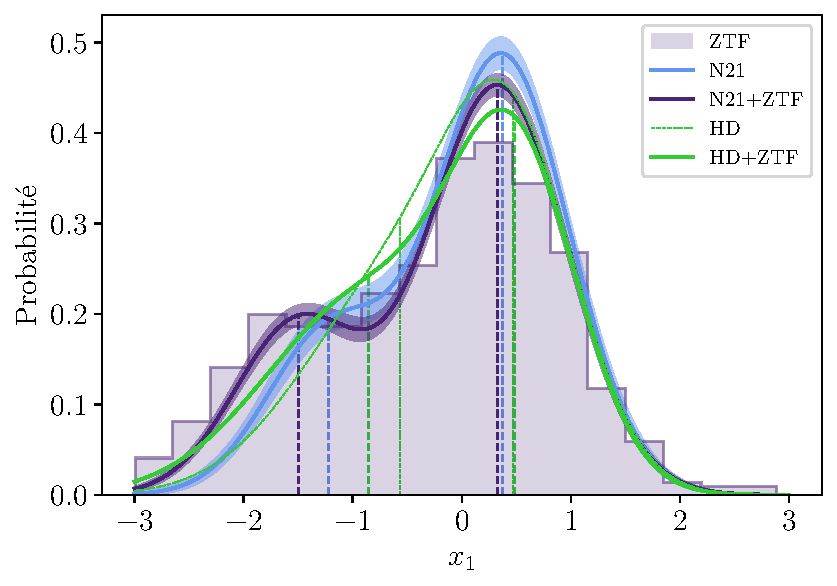
\includegraphics[width=.6\linewidth]{model_N21+HD+ZTF_on_ZTF}
    \caption[Accord entre les modèles N21+ZTF et HD+ZTF et l'histogramme des
    étirements de ZTF]{\textit{En violet}~: histogramme des étirements de ZTF.
        \textit{En bleu (violet) et leurs bandes}~: modèles de base ajustés sur
        l'échantillon de base, N21 (échantillon avec ZTF, N21+ZTF) au redshift
        moyen de ZTF et leur erreur. \textit{En fin pointillés verts (ligne
        continue)}~: modèles Howell+dérive ajustés sur l'échantillon de base, HD
    (échantillon avec ZTF, HD+ZTF).}
    \label{fig:N21HDZTFerr}
\end{SCfigure}

Nous remarquons que s'il existe bien un pic de petit étirement, le modèle N21 ne
le caractérise que partiellement, la distribution du modèle étant écartée
d'environ \num{0.30} de ce que nous pourrions considérer comme la moyenne de ce
mode de petit étirement. Il reste bien plus proche que le modèle Howell+dérive
ajusté sur l'échantillon de base (ci-après HD), représenté en fins pointillés
verts Figure~\ref{fig:N21HDZTFerr}.

\subsection{Implémentation}\label{ssec:xamel}

Nous constatons que même si le sondage SNf a permis l'établissement d'un modèle
robuste \textit{via} l'utilisation du LsSFR comme traceur de l'âge, le manque de
données à bas redshift limite la force de ces résultats. C'est pourquoi nous
proposons d'inclure les données de ZTF dans cette étude. Les résultats de
l'ajustement de ce modèle à l'ensemble des 1207 (respectivement 815) SNe~Ia de
l'échantillon fiduciel+ZTF (conservatif+ZTF) sont présentés dans le
Tableau~\ref{tab:modelresults_ztf}. Comme attendu, les paramètres du mode de
grand étirement $(\mu_1,\sigma_1$) ne diffèrent pas significativement des
résultats précédents, mais la moyenne du mode de petit étirement $\mu_2$ est
bien plus basse et écartée de $\approx 3\sigma$ des résultats de base. Nous
pouvons également noter une baisse de l'amplitude du mode 1 dans la combinaison
linéaire composant la distribution sous-jacente de la vieille population,
donnant donc plus d'amplitude au mode de petits étirements.

\begin{table*}
    \centering
        \caption[Valeurs des paramètres du modèle d'étirement de base selon
        l'échantillon avec les données de ZTF]{Valeurs des paramètres issus des
            meilleurs ajustements du modèle de distribution de l'étirement de
            base lorsqu'il est appliqué à l'ensemble de données fiduciel
            seulement (569 SNe~Ia), à l'échantillon fiduciel avec ZTF (1207) ou
        à l'échantillon conservatif avec ZTF (815).}
        \label{tab:modelresults_ztf}
    \begin{threeparttable}
        \makebox[\linewidth]{%
        \begin{tabular}{lccccc}
            \toprule
            Échantillon      & $\mu_1$             & $\sigma_1$
                             & $\mu_2$             & $\sigma_2$
                             & $a$ \\
            \midrule
            Fiduciel         & $ 0.37 \pm 0.04$    & $0.61 \pm 0.03$
                             & $-1.22 \pm 0.11$    & $0.56 \pm 0.07$
                             & $ 0.51 \pm 0.07$ \\
            Fiduciel+ZTF     & $ 0.33 \pm 0.03$    & $0.64 \pm 0.02$
                             & $-1.50 \pm 0.06$    & $0.58 \pm 0.04$
                             & $ 0.45 \pm 0.04$ \\
            Conservatif+ZTF  & $ 0.35 \pm 0.03$    & $0.61 \pm 0.02$
                             & $-1.50 \pm 0.06$    & $0.54 \pm 0.04$
                             & $ 0.45 \pm 0.04$ \\
            \bottomrule
    \end{tabular}}
        \begin{tablenotes}[flushleft]
            \item\small \textbf{\hspace{-3.2pt}Notes.} La différence principale se
                situe sur la position de la moyenne du mode de bas étirement,
                $\mu_2$, complètement incompatible avec la moyenne résultant de
                l'ajustement avec les données de base. Nous notons également
                l'augmentation de l'amplitude de ce mode \textit{via} la
                réduction du paramètre $a$ décrivant l'amplitude relative des
                deux modes dans la distribution sous-jacente de la population
                vieille.
        \end{tablenotes}
    \end{threeparttable}
\end{table*}

Le modèle de base ajusté sur l'échantillon incluant les données de ZTF est
ci-après nommé N21+ZTF, de même pour le modèle Howell+dérive qui sera nommé
HD+ZTF. Nous donnons Figure~\ref{fig:N21HDZTFerr} les représentations graphiques
de ces quatre distributions au redshift moyen des données de ZTF. Nous
constatons que le modèle N21+ZTF possède alors un second pic de bas étirements
plus éloigné en moyenne que le modèle N21, donnant un meilleur ajustement quand
nous le comparons à l'histogramme des étirements de ZTF, comme attendu. Le modèle
HD+ZTF bénéficie aussi de l'inclusion de ces données, sa moyenne de petits
étirements étant plus proche de la valeur centrale de ce pic. Llle reste
cependant toujours plus éloignée que celle définie par le modèle N21. Les
évolutions prédites de l'étirement avec le redshift ($x_1$ attendu compte tenu
de la distribution de l'équation~\ref{eq:stretchz}) sont illustrées sous la
forme d'une bande violette pour N21+ZTF et bleue pour N21 dans la
Figure~\ref{fig:evol_all_ztf}, qui tiennent compte des erreurs des paramètres et
de leurs covariances. Cette figure montre que l'étirement moyen mesuré des
SNe~Ia par intervalle de redshift (contenant tous le même nombre de données
selon l'échantillon utilisé pour l'ajustement) suit de près notre modélisation
de la dérive avec le redshift. Cependant, les deux modèles N21 et N21+ZTF ne
sont pas compatibles entre eux. Nous avons également représenté les évolutions
des modèles HD et HD+ZTF en vert pointillé et plein respectivement. Alors que
dans la Figure~\ref{fig:N21HDZTFerr} la moyenne du mode de petit étirement de
HD+ZTF se rapproche plus du pic de la distribution de ZTF que celle de HD, il
s'écarte beaucoup plus du modèle de base ajusté sur l'échantillon combiné que ce
dernier. Alors que dans N21, ce modèle était relativement compatible avec le
modèle de référence, l'ajout des données de ZTF le rend incompatible avec le
modèle de base. 

\begin{figure}[ht]
    \centering
    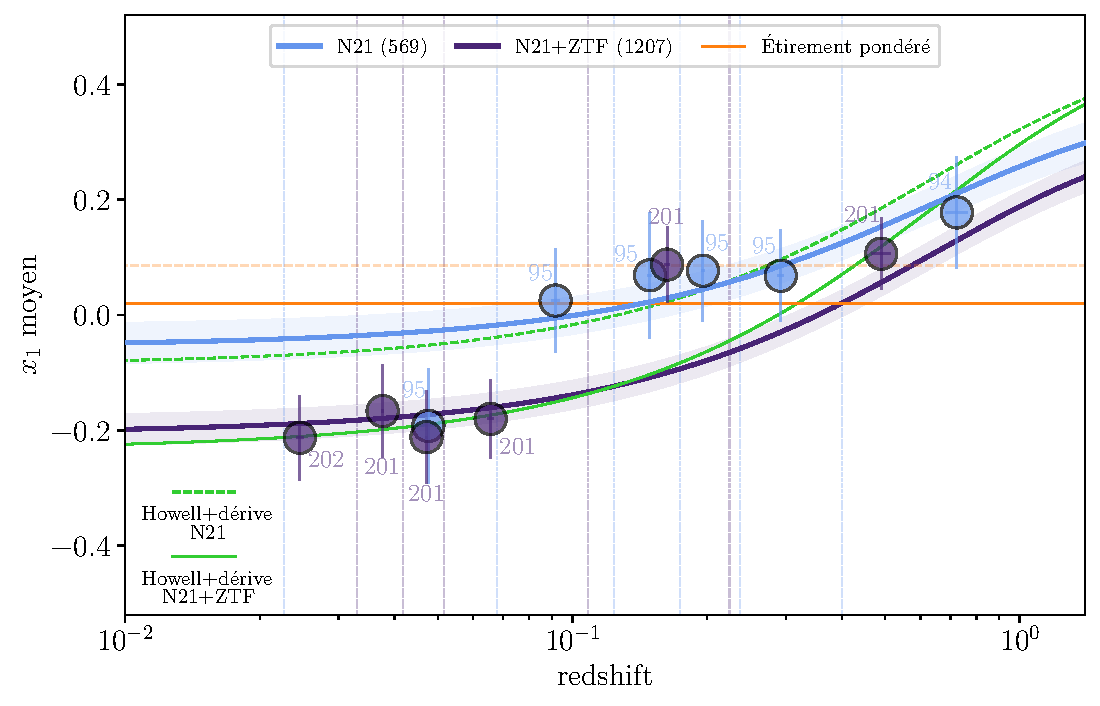
\includegraphics[width=1\linewidth]{stretchevol_all-oth_vs_ztf-weighted.pdf}
    \caption[Évolution de l'étirement moyen des SNe~Ia en fonction du redshift
    issu de la prédiction de notre modèle de base selon l'échantillon
    utilisé]{\footnotesize \textit{En bleu (et sa bande)}~: évolution de
        l'étirement moyen ($x_1$) des SNe~Ia en fonction du redshift pour notre
        modèle de base ajusté sur les données de base, nommé N21 (et son
        erreur). \textit{En violet (et sa bande)}~: même modèle mais ajusté sur
        les données de base combinées aux données de ZTF, nommé N21+ZTF (et son
        erreur). Ces deux modèles ne sont pas compatibles entre eux. Les
        marqueurs montrent la moyenne pondérée de l'étirement mesurée dans des
        intervalles de redshift de tailles d'échantillon égales pour chaque
        ensemble de données, indiquées en \textit{bleu clair} et en
        \textit{violet clair} à côté de chaque point de mesure pour les modèles
        N21 et N21+ZTF, respectivement. La \textit{ligne horizontale orange
        pleine (pointillée)} représente l'étirement pondéré des données.
        \textit{La ligne verte (pointillée)} représente le meilleur ajustement
        du modèle Howell+dérive ajusté sur l'échantillon fiduciel combiné à ZTF
        (fiduciel de base). Alors que dans N21, ce modèle était relativement
        compatible avec le modèle de référence, l'ajout des données de ZTF le
    rend incompatible avec le modèle de référence.}
    \label{fig:evol_all_ztf}
\end{figure}

\subsection{Résultats}\label{ssec:zres}

Nous présentons les résultats quantitatifs de cette étude sous la même forme que
précédemment, à l'aide du Tableau~\ref{tab:comp_ztf}, illustré par le graphique
Figure~\ref{fig:mod_comp_ztf}.

\newgeometry{margin=1cm}
\begin{landscape}
% \sidecaptionvpos{figure}{c}
\begin{SCfigure}[.5][p]
%    \centering
    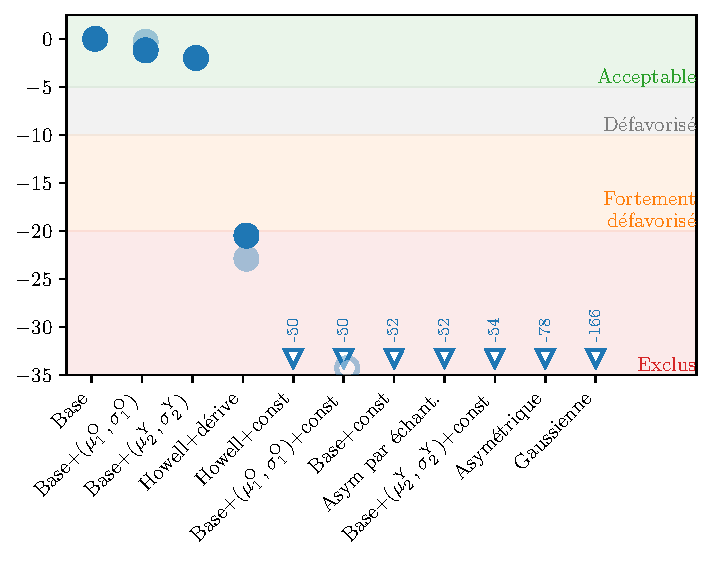
\includegraphics[width=.40\linewidth]{mod_comp_ztf-fr}
    \caption[$\Delta$AIC entre le modèle de base et les autres
    modèles]{$\Delta$AIC entre le modèle de référence et les autres modèles en
        utilisant les données de ZTF (voir Tableau~\ref{tab:comp_ztf}). La
        légende suit celle de la Figure~\ref{fig:mod_comp}. En suivant ces
        valeurs d'AIC, tous les modèles sans dérive (marqueurs ouverts) sont
        exclus car il représentent moins bien les données que le modèle de
    référence, avec dérive.}
    \label{fig:mod_comp_ztf}
\end{SCfigure}
% \sidecaptionvpos{figure}{t}

\begin{table}[p]
    \centerfloat
    \thisfloatpagestyle{empty}
    \caption[Comparaison de la capacité relative de chaque modèle à décrire les
    données par rapport au modèle de base avec les données de ZTF]{Comparaison
        de la capacité relative de chaque modèle à décrire les données en
    utilisant les données de ZTF} \label{tab:comp_ztf}
    \begin{threeparttable}
        \makebox[\linewidth]{
        \begin{tabular}{lcccccccc}
            \toprule
            & & & \multicolumn{3}{c}{Échantillon fiduciel+ZTF (1207 SNe)}
                & \multicolumn{3}{c}{Échantillon conservatif+ZTF (815 SNe)} \\
            \cmidrule(lr){4-6} \cmidrule(lr){7-9}
            Nom & dérive & $k$ &
            $-2\ln(L)$ & AIC & $\Delta$AIC & $-2\ln(L)$ & AIC & $\Delta$AIC\\
            \midrule
            % Quad. Gauss & $\delta(z)$ & 10
            % & 3344,0 & 3364,0 & 2,5 
            % & 2204,7 & 2224,7 & 8,6 \\
            Base & $\delta(z)$ & 5
            & 3348,7 & 3358,7 & -- 
            & 2215,5 & 2225,5 & -- \\
            Base+$(\mu_1^{\rm O},\sigma_1^{O})$ & $\delta(z)$ & 7
            & 3345,9 & 3359,9 & -1,2 
            & 2211,8 & 2225,8 & -0,3 \\
            Base+$(\mu_2^{\rm Y},\sigma_2^{Y})$ & $\delta(z)$ & 6
            & 3348,7 & 3360,7 & -2,0 
            & 2215,5 & 2227,5 & -2,0 \\
            Howell+dérive & $\delta(z)$ & 4
            & 3371,1 & 3379,1 & -20,5
            & 2240,4 & 2248,4 & -22,9 \\
            Howell+constant & $f$ & 5
            & 3398,3 & 3408,3 & -49,6
            & 2252,8 & 2262,8 & -37,2 \\
            Base+$(\mu_1^{\rm O},\sigma_1^{O})$+const & $f$ & 8
            & 3393,1 & 3409,1 & -50,4
            & 2243,8 & 2259,8 & -34,3 \\
            Base+const & $f$ & 6
            & 3398,3 & 3410,3 & -51,6
            & 2252,8 & 2264,8 & -39,2 \\
            Asym.\ par échant. & Par échant. & 3$\times$6
            & 3374,3 & 3410,3  & -51,7
            & 2240,9 & 2276,9  & -51,3 \\
            Base+$(\mu_2^{\rm Y},\sigma_2^{Y})$+const & $f$ & 7
            & 3398,3 & 3412,3 & -53,6
            & 2252,8 & 2266,8 & -41,2 \\
            % Quad. Gauss+const & $f$ & 11
            % & 3392,3 & 3414,3 & -55,6
            % & 2248,9 & 2270,9 & -37,6 \\
            Asymétrique & -- & 3
            & 3431,1 & 3437,1 & -78,5
            & 2278,3 & 2284,3 & -58,8 \\
            Gaussienne & -- & 2
            & 3520,5 & 3524,5 & -165,8
            & 2365,6 & 2369,6 & -144,0 \\
            \bottomrule
        \end{tabular}}
        \begin{tablenotes}[flushleft]
            \item\small \textbf{\hspace{-3.2pt}Notes.} Pour chaque modèle
                considéré, nous indiquons si le modèle dérive ou non ainsi que
                son nombre de paramètres libres $k$. Nous renseignons les
                valeurs de, $-2\ln(L)$ (voir Équation~\ref{eq:likelihood}),
                l'AIC et la différence d'AIC ($\Delta$AIC) pour les échantillons
                fiduciel et conservatif entre ce modèle et le modèle de base,
                choisi comme référence car présentant l'AIC le plus faible.
        \end{tablenotes}
    \end{threeparttable}
\end{table}
\end{landscape}
\restoregeometry

Nous voyons ici que l'incompatibilité visuelle entre HD+ZTF et N21+ZTF se
traduit très fortement au niveau de la différence d'AIC. En effet, nous
remarquons d'abord que le modèle de base s'établit encore comme le modèle de
référence. Les différentes variations au modèle de la
Section~\ref{ssec:testsupp} restent proches du modèle de base, mais sont
toujours défavorisées par l'AIC. En revanche, cette fois ci l'écart d'AIC avec
le modèle Howell+dérive est de 20,7, excluant cette modélisation comme bonne
représentation des données par rapport au modèle de base. L'exclusion des
modèles non-dérivants est également renforcée, le premier modèle non-dérivant
ayant un AIC plus petit de 49,7 par rapport à notre modèle de référence, et plus
petit de 29,2 comparé à Howell+dérive. Le modèle asymétrique pur est toujours
exclu, mais cette fois rendu à l'avant-dernière place du classement.

Bien que l'ajout de ces données apporte plus de robustesse aux conclusions
principales sur la dérive de l'étirement avec le redshift, nous nous
interrogeons sur la qualité de ces nouveaux paramètres à décrire les
échantillons déjà existants. Pour cela, nous avons calculé la quantité
$-2\ln(L)$ pour chacun des modèles N21 et N21+ZTF, ajustés sur leurs
échantillons respectifs, quand nous les comparons aux données des sondages. La
Figure~\ref{fig:bzcomp} et le Tableau~\ref{tab:bzcomp} résument ces résultats.

\begin{figure}[p]
    \centerfloat
    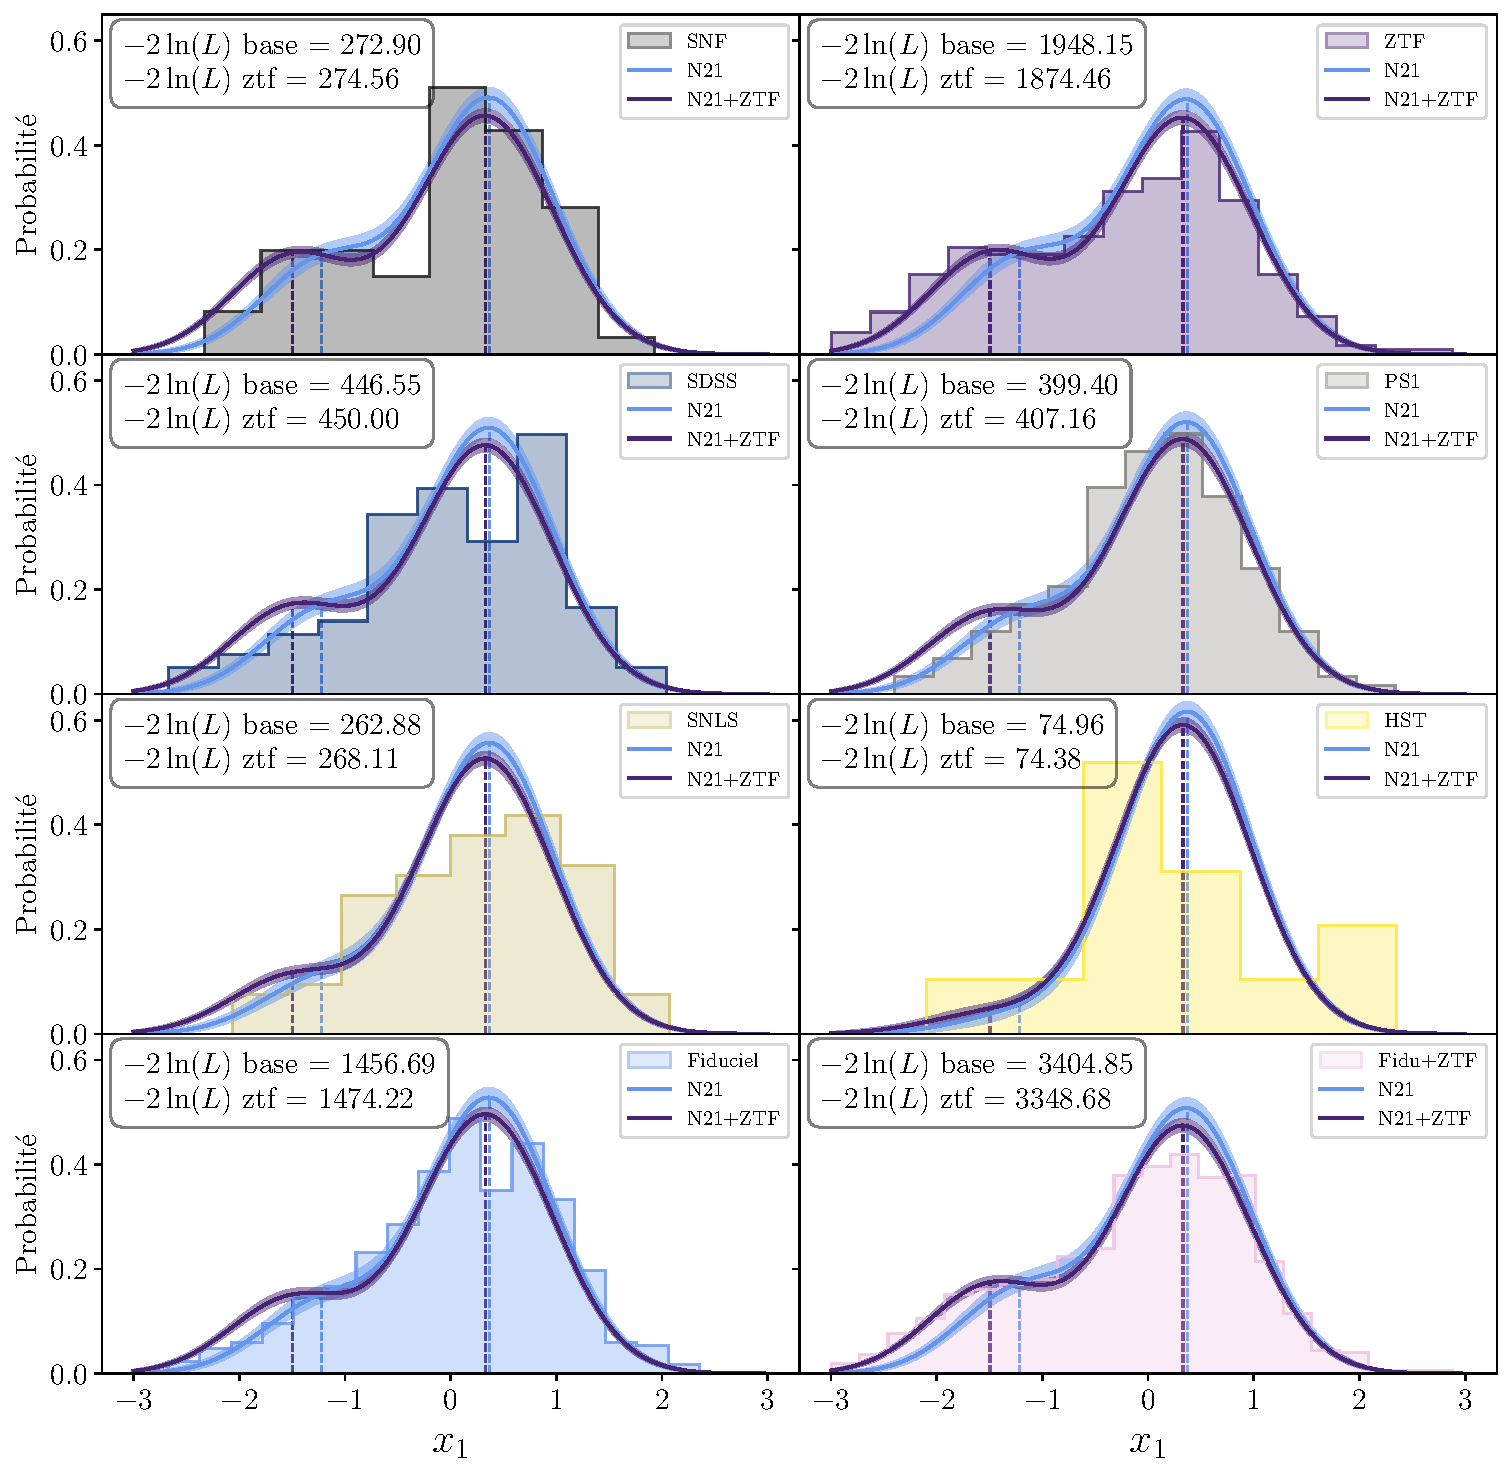
\includegraphics[width=1\linewidth]{model_N21+ZTF_on_allsurvs}
    \caption[Comparaison de la capacité des modèles N21 et N21+ZTF à représenter
    les données des sondages]{Comparaison de la capacité des modèles N21 et
    N21+ZTF à représenter les données des sondages. Pour chaque sondage, nous
traçons l'histogramme correspondant et les modèles N21 et N21+ZTF au redshift
moyen dudit sondage en ligne (et bande) bleue et violette respectivement (et
leurs erreurs). Le modèle N21 présente un meilleur ajustement pour chacun des
sondages sauf pour ZTF, rendant l'accord bien plus qualitatif quand ce dernier
est inclus dans l'échantillon total que quand il ne l'est pas.}
    \label{fig:bzcomp}
\end{figure}

\begin{table}[ht]
    \centering
        \caption[Capacité des modèles N21 et N21+ZTF à représenter les
        données]{Valeurs des quantités $-2\ln(L)$ des modèles N21 et N21+ZTF par
        sondage.}
        \label{tab:bzcomp}
    \begin{threeparttable}
        \makebox[\linewidth]{%
        \begin{tabular}{lcccccccc}
            \toprule
            & \multicolumn{8}{c}{Sondage}\\
            \cmidrule(lr){2-9}
            Modèle & SNF & ZTF & SDSS & PS1 & SNLS & HST & Base & Base+ZTF\\
            \midrule
            N21 &
            272,9 & 1948,2 & 446,6 & 399,4 & 262,9 & 75,0 & 1456,7 & 3404,9\\
            N21+ZTF & 
            274,6 & 1874,5 & 450,0 & 407,2 & 268,1 & 74,4 & 1474,2 & 3348,7\\
            Variation &
            1,66 & -73,69 & 3,45 & 7,76 & 5,23 & -0,57 & 17,53 & -56,16\\
            \bottomrule
    \end{tabular}}
        \begin{tablenotes}[flushleft]
        \item\small \textbf{\hspace{-3.2pt}Notes.} N21 correspond au modèle de
            base ajusté sur l'échantillon fiduciel de base. N21+ZTF correspond
            au même modèle mais ajusté sur l'échantillon fiduciel de base
            combiné à celui de ZTF.
        \end{tablenotes}
    \end{threeparttable}
\end{table}

Nous observons que le modèle N21 présente une meilleure capacité à décrire les
données qui ne sont pas ZTF, avec une différence de $-2\ln(L)$ augmentant de SNf
à PS1 où nous trouvons une différence de 7,76 en faveur de N21, avant de
redescendre jusqu'à une différence de -0,57 en faveur de N21+ZTF. En revanche,
chaque modèle présente une meilleure capacité à décrire son échantillon que
l'autre, comme attendu. Nous pouvons avancer que l'intégration de ce nouvel
ensemble de données, statistiquement supérieur au précédent et sur une plage
limitée de redshift, biaise la capacité du modèle à représenter les données en
lui imposant de reproduire les caractéristiques de cet échantillon particulier.
Nous insistons cependant sur le fait que ces données sont préliminaires,
contenant notamment des SNe~Ia n'était pas de qualité cosmologique ayant une
tendance à présenter des étirements particulièrement bas~; ces résultats sont
donc encourageants pour la présence d'une distribution avec deux pics
d'étirements d'amplitude relative correcte, et le travail nécessaire qui suivra
permettra sans doute d'améliorer cette étude.

\subsection{Conclusion}\label{ssec:ztfconc}

Grâce au début de publication des résultats du nouveau sondage ZTF, nous avons
pu étendre l'étude initiale du Chapitre~\ref{ch:stretch} et créer un nouveau
sous-échantillon limité en volume, faisant passer notre échantillon combiné de
569 à 1207 SNe~Ia (et de 422 à 815 avec les coupes conservatives). Ainsi, compte
tenu de l'ensemble de données actuel, nous suggérons l'utilisation du modèle de
population d'étirements évoluant avec le redshift suivant~:
\begin{align*}\label{eqconclusion:stretchz}
    X_1\left(z \right) =
        \delta(z)&\times\mathcal{N}(\mu_1,\sigma_1{}^2)\,+\nonumber\\
        (1-\delta(z))&\times \left[a\times\mathcal{N}(\mu_1,\sigma_1{}^2) +
        (1-a)\times\mathcal{N}(\mu_2,\sigma_2{}^2)\right],
    \tag{\ref{eq:stretchz}}
\end{align*}
avec $a=0.45$, $\mu_1=0.33$, $\mu_2=-1.50$, $\sigma_1=0.64$, et $\sigma_2=0.58$
(voir Tableau~\ref{tab:modelresults_ztf}), et d'utiliser le modèle de dérive
de la population d'âge avec le redshift suivant~:
\begin{align*}
    \delta(z) & = \left( K^{-1} \times (1+z)^{-2.8} +1 \right)^{-1}
    \tag{\ref{eq:deltaz}}
\end{align*}
avec $K=0.87$.

Au travers de l'ajout des données de ZTF à notre étude, nous avons pu rendre
plus robuste la conclusion selon laquelle les modèles d'étirements des SNe~Ia
n'incluant pas de dérive avec le redshift étaient tous exclus en tant que bonnes
représentations de données par rapport aux modèles dérivants, mais nous avons
également renforcé la pertinence du modèle de base à cet effet. Si l'accord sur
les autres sondages est moindre que précédemment, nous pouvons nous attendre à
ce que des données telles que celles du LSST à moyen redshift ou Subaru à haut
redshift permettent de rééquilibrer cette différence statistique sur la plage de
redshifts sondés pour continuer d'améliorer cette définition de
sous-populations, tout en continuant à utiliser les qualités du sondage ZTF à
cet effort.

\section{Simulations~: améliorations}\label{sec:simpersp}

Dans le chapitre précédent, nous avons implémenté le premier modèle d'étirement
à l'ensemble de logiciels \snana. Bien que les résultats de ces simulations
soient concluants, nous proposons différentes approches et perspectives qui
permettraient d'étendre ces analyses.

\subsection{Types de simulations}\label{ssec:types}

Nous pouvons implémenter différentes manières d'effectuer ces simulations, que
nous appelons «~types~».

En premier lieu, nous pourrions réduire les incertitudes statistiques de
l'approche précédente en augmentant le nombre de données simulées. Ceci
demanderait en retour d'augmenter considérablement la taille de l'échantillon de
BiasCor, déjà proche de $10^6$ données mais qui ne permet pourtant pas de
corriger l'intégralité des SNe des données simulées ($\approx 15\%$ n'ont pas de
BiasCor).

Pour étudier l'impact des modélisations sur l'état de la cosmologie actuelle,
une approche possible serait de simuler une grand nombre de fois ($\approx
\num{100}$) des échantillons de la taille de l'échantillon de Pantheon ($\approx
\num{1000}$) et de combiner les résultats, permettant ainsi d'avoir des
incertitudes statistiques réalistes.

Ces types et des variations ont été implémentées, mais la complexité des
simulations avec \snana\ nous ont amenæ à modifier les paramètres de simulation
jusqu'au dernier moment, rendant impossible le fait d'effectivement réaliser ces
types de simulations, bien que cela reste à notre portée dans l'avenir.

\subsection{Variation de paramètres}\label{ssec:pvar}

Avec l'ajout des données de ZTF, notre modèle d'évolution de l'étirement avec le
redshift a été augmenté. Ces nouveaux paramètres pourraient être utilisés,
notamment pour tenter de représenter plus efficacement l'échantillon ciblé LOWZ
qui présente un pic de petits étirements autour de $x_1 \approx -1.50$. À cet
effet, nous pourrions utiliser non pas le redshift de l'échantillon mais
directement la fraction attendue pour décrire l'étirement de la \hostlib\
utilisée pour simuler cet échantillon~; cette approche briserait en quelque
sorte l'approche prospective de notre étude, mais apparaît comme nécessaire pour
simuler des données elles-mêmes sélectionnées.

Dans toute cette thèse, nous avons utilisé l'équation de l'évolution de la
fraction de jeunes étoiles $\delta(z)$ donnée dans le Chapitre~\ref{ch:env},
avec les résultats des paramètres $K$ et $\phi$ de~\cite{rigault2020}. Ceux-ci
pourraient être variés, notamment le paramètre $K$ qui est obtenu pour fixer la
fraction de jeunes étoiles à 50\% à $z = \num{0.05}$.

\subsection{Traceurs environnementaux}\label{ssec:envtrac}

Comme nous avons pu le voir, l'ajout du traceur de l'âge d'une SN permettrait
d'augmenter la robustesse de notre étude et pourrait s'avérer être un outil
probant des propriétés intrinsèques des SNe~Ia. Nous pourrions étendre encore
plus ces analyses en intégrant d'autres traceurs utilisés en cosmologie, comme
la couleur locale.

En plus des effets environnementaux des SNe~Ia dont nous avons pu discuter
Chapitre~\ref{ch:env}, de récentes études \citep{brout2021} proposent
d'intégrer les effets de rougissement dus à la poussière des galaxies
conjointement aux variations intrinsèques des couleurs des SNe~Ia dans le modèle
\texttt{SALT2}. Ceci a permis de mieux décrire les propriétés des SNe les plus
rouges, et propose une approche pour décrire la marche de magnitude basée sur la
masse, causée par une différence sur le paramètre $\beta$ effectif selon la
masse des galaxies hôtes. \cite{popovic2021b} ont intégré cette approche à leurs
simulations pour établir une approche prospective de détermination des
distributions mères de poussière et de couleur, et trouvent une incertitude
systématique due à ces effets de \num{0.005} sur la mesure de $w$. Ces résultats
sont prometteurs quant aux perspectives d'amélioration de la recherche sur les
effets des propriétés des galaxies hôtes sur les échantillons de SNe~Ia, et
pourraient à terme amener à une modélisation continue de dépendance avec la
masse des galaxies hôtes, en lieu et place de la modélisation en marche de
magnitude utilisée aujourd'hui. L'inclusion de ces approches rendrait alors
notre étude plus consistante.

\clearpage

\thispagestyle{plain}
\vspace*{\fill}
\minilof
\vspace*{\fill}
\minilot
\vspace*{\fill}

% \bibliographystyle{../main/aa_url}
% \shorthandoff{:}
% \bibliography{../chapters/99_references}

\end{document}
